\chapter{Relaciones de Recurrencia}

Una \emph{relación de recurrencia} (o, simplemente, \emph{recurrencia})
es una función expresada en términos de sí misma, pero con una entrada
más pequeña. Las recurrencias se presentan al analizar la
eficiencia de algoritmos de tipo \emph{divide y vencerás}. La \emph{forma
cerrada} de una recurrencia es una función equivalente, pero expresada
sin recursividad. \emph{Resolver} una recurrencia implica encontrar
su forma cerrada.

En el contexto de los algoritmos divide y vencerás, las recurrencias
suelen tener la sig. forma general: 

\[
    T(n)=\begin{cases}
        \sum_{i=1}^{p}T(n_{i})+f(n) & \text{para }n>b\\
        g(n) & \text{en caso contrario}
    \end{cases}
\]
donde

\begin{itemize}
    \item $b\in\mathbb{N}$ es la condición de paro (boundary condition); esto
    es, el valor que debe tener $n$ para entrar al caso base
    \item $g:\mathbb{N}\to\mathbb{N}$ es el tiempo de ejecución del caso base
    \item $p\in\mathbb{N}$ es la cantidad de subproblemas en las que se dividió
    la entrada
    \item $n_{i}\in\mathbb{N}$, tal que $n_{i}<n$, es el tamaño de la entrada
    para el subproblema $i$ 
    \item $f:\mathbb{N}\to\mathbb{N}$ es el tiempo de ejecución para dividir
    la entrada en, y/o combinar las soluciones de los, $p$ subproblemas
\end{itemize}

En general, la función $g$ suele ser una función constante, por lo que suele omitirse. 
Esto es porque un algoritmo comúnmente alcanza su condición de paro cuando $n$ es 
es de un tamaño determinado. Por otro lado, los pisos y los techos también suelen 
omitirse. Esto es porque casi siempre se puede suponer que $n$ se puede dividir en 
en partes enteras, sin que ello afecte la cota del tiempo de ejecución.

A continuación se presentan diferentes métodos para resolver recurrencias.

\section{El método del árbol recursivo}

El método del árbol recursivo es un método gráfico e informal que
consiste de dibujar un árbol donde cada sub-árbol representa el
tiempo total requerido para resolver un subproblema en la recurrencia. Al
sumar el tiempo de todos los nodos del árbol, se obtiene la forma
cerrada de la recurrencia. Antes de estudiar el método en sí, es 
importante recordar algunos conceptos sobre árboles. 

Sea $k\in\mathbb{N}_0$, un árbol \textit{k-ario} es un árbol 
enraizado donde cada nodo tiene a lo más $k$ hijos. Se dice que un
árbol $k$-ario es \textit{lleno} si cada nodo
tiene exactamente 0 o $k$ hijos. Un árbol $k$-ario 
\textit{perfecto} es un árbol $k$-ario lleno donde todas las hojas 
están en el mismo nivel. 

La \textit{profundidad} de un nodo es la distancia entre dicho nodo 
y la raíz. Por definición, el nodo raíz tiene una profundidad de 0. 
En un árbol $k$-ario perfecto, el número de vértices a 
profundidad $d$ está dado por $k^d$. Para terminar, la \textit{altura} 
de un árbol es la profundidad más grande de todos los nodos del árbol. 
Así, la altura de un árbol $k$-ario perfecto de $n\in\mathbb{N}$ 
nodos está dado por $\log_k{n}$.

El método del árbol recursivo consiste de los sig. pasos:

\begin{enumerate}
    \item Se desglosa la recurrencia en un árbol de tal forma que la raíz representa
    el tiempo requerido para combinar y/o dividir el problema original,
    cada nodo interno representa el tiempo requerido para combinar y/o
    dividir un subproblema y cada hoja representa el tiempo requerido
    por el caso base. 
    \item Se calcula la cantidad de niveles en el árbol.
    \item Se calcula la cantidad de hojas.
    \item Para cada nivel, se suman los valores de los nodos que contiene.
    \item Se suma el tiempo total de todos los niveles para obtener la
    forma cerrada.
\end{enumerate}
Las expresiones obtenidas en los pasos 2, 3 y 4 
se definen en función de $n$ y la expresión obtenida en el paso 5 normalmente consiste de 
una sumatoria que debe resolverse para obtener la forma cerrada.

Si se tiene una recurrencia la forma $T(n)=aT(n/b)+f(n)$, donde $a,b\in\mathbb{N}$ y 
$f:\mathbb{N}\to\mathbb{N}$ es una función asintóticamente 
positiva, intuitivamente se puede ver que $a$ indica 
la cantidad de hijos que tendrá cada nodo en árbol recursivo, $b$ indica qué tanto se reduce 
el tamaño del problema en cada nivel y $f(n)$ es el valor que tendrá cada nodo en el árbol.

\begin{expl}
    Considérese la recurrencia $T(n)=3T(\lfloor n/4 \rfloor)+\Theta(n^2)$. 
    Antes de comenzar, vale la pena simplificar $T(n)$. Se
    puede suponer que $n$ es un múltiplo de 4, para así ignorar el piso, y se puede 
    sustituir $\Theta(n^2)$ por $cn^2$, donde $c\in\mathbb{R}$ es 
    una constante. Así, se obtiene la recurrencia $T(n)=3T(n/4)+cn^2$. 
    El sig. paso es dibujar el árbol recursivo de esta recurrencia. La figura 
    \ref{recursion-tree} muestra cómo dibujar dicho árbol y cómo obtener la forma cerrada a 
    partir de él.
    
    Una vez dibujado el árbol, se debe calcular la altura y el número de hojas. 
    Dado que el valor de $n$ se reduce en $1/4$ en cada nivel, se requiere iterar 
    $\log_4{n}$ veces para llegar a $n=1$, que constituye la condición de paro de la 
    recurrencia. Así, se tiene que la altura del árbol es $\log_4{n}$ y el número de 
    hojas está dado por $3^{\log_{4}{n}}=n^{\log_{4}{3}}$.
    
    Para calcular el tiempo total de cada nivel, hay que recordar que cada nodo tiene
    tres hijos y que su valor es $cn^2$, donde $n$ se va reduciendo en un factor fijo. 
    Así, se puede deducir que el tiempo total 
    de cada nivel está dado por $(3/16)^i\cdot cn^2$, donde $i\in\mathbb{N}_0$
    representa la profundidad de cada nivel. Obsérvese que esta expresión aplica para todos 
    los niveles excepto el último, pues el tiempo del último nivel depende del caso base. 
    En este ejemplo, el tiempo del último nivel está dado por
    $n^{\log_{4}{3}}T(1)=\Theta(n^{\log_{4}3})$ (suponiendo que $T(1)$ es una constante).
    
    Por último, se suman los tiempos de todos los niveles, cosa que para este ejemplo 
    resulta en la sig. expresión:
    
    \begin{align*}
        T(n)&=\sum_{i=0}^{\log_{4}n-1}\left(\dfrac{3}{16}\right)^{i}\cdot cn^{2}+\Theta(n^{\log_{4}3}) \\
    	&<\sum_{i=0}^{\infty}\left(\dfrac{3}{16}\right)^{i}\cdot cn^{2}+\Theta(n^{\log_{4}3}) \\
    	&=\dfrac{1}{1-3/16}\cdot cn^{2}+\Theta(n^{\log_{4}3}) \\
    	&=\dfrac{16}{13}\cdot cn^{2}+\Theta(n^{\log_{4}3}) \\
    	&=O(n^{2})+O(n^{\log_{4}3}) \\
    	&=O(n^{2})
	\end{align*}
	\exend
\end{expl}

\begin{figure}[H]
\begin{centering}
    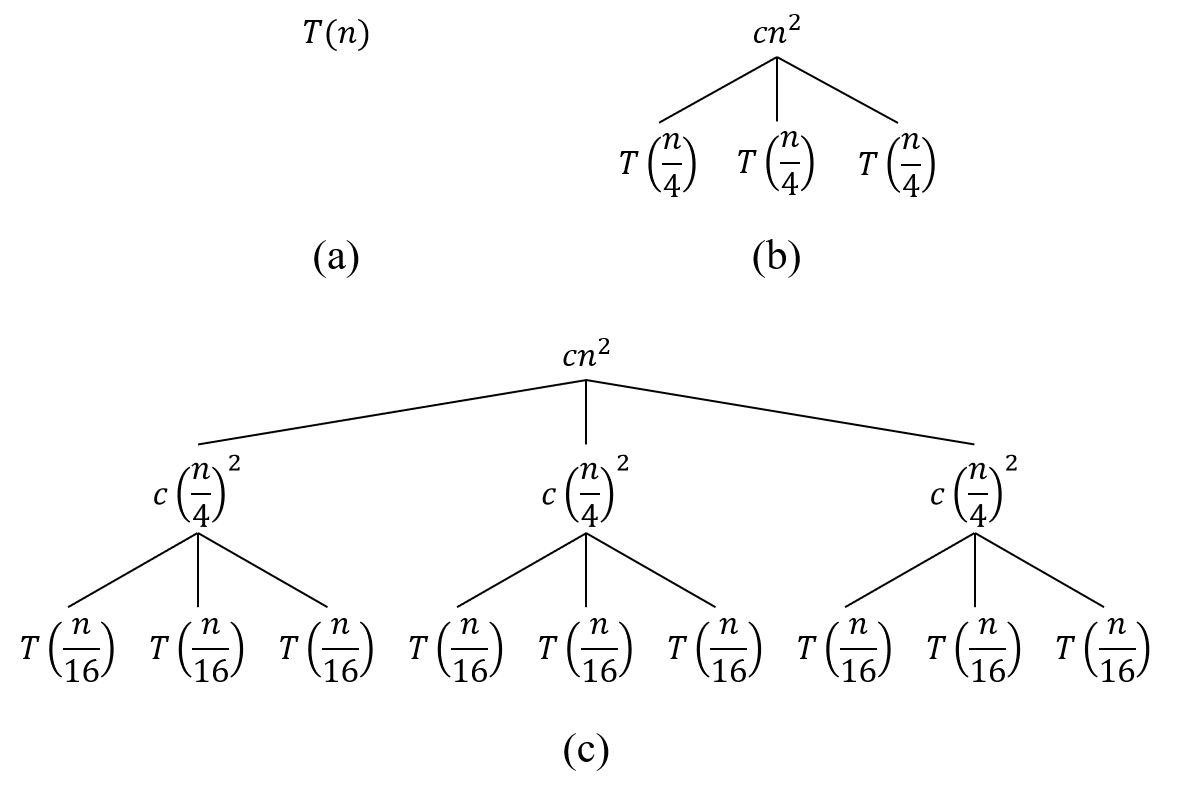
\includegraphics[width=0.75\textwidth]{figuras/recursion-tree1}
    \par\end{centering}
    \begin{centering}
    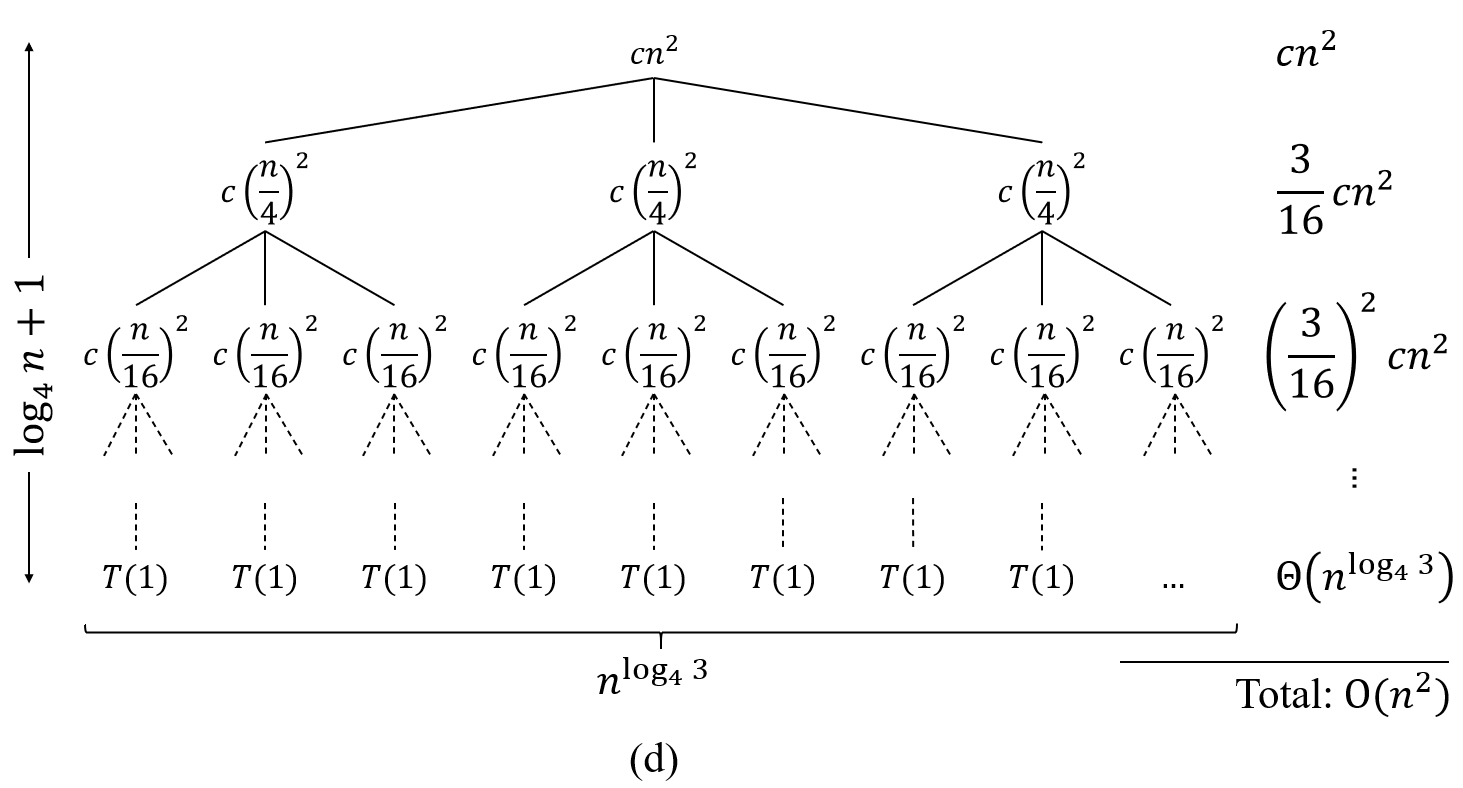
\includegraphics[width=1\textwidth]{figuras/recursion-tree2}
    \par\end{centering}
    \caption{{\small{}\label{recursion-tree}Usando el método del árbol recursivo para
    resolver la recurrencia $T(n)=3T(n/4)+cn^{2}$. (a)-(c) Desgloce
    del árbol, comenzando con la raíz y continuando con los hijos en cada nivel. 
    (d) Calculando el número de nodos en cada nivel y sumándolos para obtener la
    forma cerrada de la recurrencia.}}
\end{figure}

\section{El método maestro}

El método maestro consiste simplemente en aplicar el teorema que se presenta a
continuación.

\begin{thm}[teorema maestro]
    Sean $a,n\in\mathbb{N}$ y $b\in\mathbb{R}$, donde $a$ y $b$ son
    constantes y $b>1$. Sea $f:\mathbb{N}\to\mathbb{N}$ una función
    asintóticamente positiva y sea $c=\log_{b}a$. Si $T:\mathbb{N}\to\mathbb{N}$
    es una recurrencia de la forma $T(n)=aT(n/b)+f(n)$, entonces se puede
    resolver aplicando uno de los sig. casos:
    \begin{enumerate}
        \item Si $f=O(n^{c-\varepsilon})$ para alguna constante real $\varepsilon>0$,
        entonces $T=\Theta(n^{c})$.
        \item Si $f=\Theta(n^{c})$, entonces $T=\Theta(n^{c}\log n)$.
        \item Si $f=\Omega(n^{c+\varepsilon})$ y si, además, $af(n/b)\leq kf(n)$
        para alguna constante real $k<1$ y para todo valor de $n$ pasado
        algún umbral, entonces $T=\Theta(f)$.
    \end{enumerate}
\end{thm}

\begin{rem}
    Para el teorema maestro, el término $n/b$ también se puede interpretar
    como $\lceil n/b\rceil$ o $\lfloor n/b\rfloor$.
\end{rem}

Una forma intuitiva de interpretar el teorema maestro es la siguiente.
La función $f$ representa el costo de combinación y/o división de los subproblemas
en cada nivel del árbol recursivo, mientras que la función $n^c$ representa
el número de hojas en dicho árbol. De estas dos funciones, aquella que creces
más rápido es la solución de la recurrencia. 

En el caso 1, se tiene que $n^c$
es más grande; i.e. el costo de resolver cada subproblema eventualmente
supera el costo de combinación y/o división. Por ende, $n^c$ es la solución de la 
recurrencia. En el caso 3, se tiene lo opuesto; $f$ crece más rápido que $n^c$.
Para aplicar este caso, $f$ debe además satisfacer lo que se conoce como
la ``condición de regularidad''.
Por último, en el caso 3 se tiene que ambas funciones, $f$ y $n^c$, tienen
la misma tasa de crecimiento y la solución es entonces el orden de crecimiento
de estas funciones multiplicada por un factor logarítmico que representa
la altura del árbol recursivo.

La desventaja del teorema maestro es que no todas las recurrencias se pueden
resolver aplicando este teorema, aunque sí se puede aplicar a la mayoría de 
las recurrencias que ocurren en la práctica.

\begin{expl}
    Sea $T(n)=9T(n/3)+n$. Aplicando el teorema maestro, se tiene que $a=9$, 
    $b=3$ y $f(n)=n$. Así, se obtiene $n^c=n^{\log_{3}{9}}=n^2$. Dado que 
    $f=O(n^{2-\varepsilon})$, donde $\varepsilon=1$, se aplica 
    el caso 1, lo que resulta en $T=\Theta(n^2)$.
    \exend
\end{expl}

\begin{expl}
    Sea $T(n)=T(2n/3)+1$. Aplicando el teorema maestro, se tiene que $a=1$,
    $b=3/2$ y $f(n)=1$. Así, se obtiene $n^c=n^{\log_{3/2}{1}}=n^0=1$.
    Dado que $f=n^c=1$, se tiene que $f=\Theta(n^c)$ y se aplica el caso 2, 
    lo que resulta en $T=\Theta(\log{n})$.
    \exend
\end{expl}

\begin{expl}
    Sea $T(n)=3T(n/4)+n\lg{n}$. Aplicando el teorema maestro, se tiene que 
    $a=3$, $b=4$ y $f(n)=n\lg{n}$. Así, se obtiene 
    $n^c=n^{\log_{4}{3}}=O(n^{0.793})$. Dado que 
    $f=\Omega(n^{\log_{4}{3}+\varepsilon})$,
    donde $\varepsilon\approx 0.2$, se aplica el caso 3 si se demuestra 
    que $f$ cumple la condición de regularidad; i.e. que $af(n/b)\leq kf(n)$,
    donde $k<1$. Para ello, se tiene que
    $3(n/4)\lg(n/4)\leq (3/4)n\lg{n}$ para valores 
    suficientemente grandes de $n$. Como consecuencia,
    se aplica el caso 3, lo que resulta en $T=\Theta(n\log n)$.
    \exend
\end{expl}

\begin{expl}
    Sea $T(n)=2T(n/2)+n\lg{n}$. El teorema maestro no se puede aplicar
    a esta recurrencia a pesar de tener la forma apropiada. Si se 
    maneja que $a=2$, $b=2$ y $f(n)=n\lg{n}$, se obtendría $n^c=n^{\log_{2}{2}}=n$.
    Dado que $f$ es asintóticamente más grande que $n^c$, se podría pensar que se puede
    aplicar el caso 3, pero no es así debido a que $f$ no es
    polinomialmente más grande que $n^c$; i.e. la razón entre $f$ y $n^c$ 
    no resulta en un polinomio.
    \exend
\end{expl}

\section{El método de Akra-Bazzi}

El método de Akra-Bazzi es una generalización del teorema maestro que admite
variables continuas y que permite resolver recurrencias donde los subproblemas 
en un mismo nivel son de diferente tamaño. El método de Akra-Bazzi trabaja 
sobre recurrencias de la sig. forma:

$$
T(x)=
\begin{cases}
    \sum_{i=1}^{k}a_iT(b_ix)+f(x) &\quad \text{si }x>x_0 \\
    \Theta(1) &\quad \text{si }1\leq x \leq x_0
\end{cases}
$$
donde
\begin{itemize}
    \item $x\geq 1$ es un número real
    \item $x_0\in\mathbb{R}$ es una constante tal que $x_0\geq 1/b_i$ y $x_0\geq 1/(1-b_i)$
    para toda $1\leq i\leq k$
    \item $a_i\in\mathbb{R^+}$ es una constante para toda $1\leq i\leq k$
    \item $b_i\in\mathbb{R^+}$ es una constante en el rango $0<b_i<1$ para toda $1\leq i\leq k$.
    \item $k\geq 1$ es una constante entera
    \item $f(x)$ es una función no negativa $f:\mathbb{R}\to\mathbb{R}_0$ que satisface
    la ``condición de crecimiento polinomial''; i.e. existen dos constantes $c_1,c_2\in\mathbb{R^+}$
    tales que, para toda $x\geq 1$, para toda $1\leq i\leq k$ y para toda $u\in\mathbb{R}$
    tal que $b_ix\leq u \leq x$, se tiene que $c_1f(x)\leq f(u)\leq c_2f(x)$
\end{itemize}
La condición de crecimiento polinomial se cumple para $f(x)$ si $|f'(x)|$ está acotada por
arriba por algún polinomio en $x$. Por ejemplo, $f(x)=x^\alpha\lg^\beta{x}$ satisface esta
condición para cualquier par de constantes reales $\alpha$ y $\beta$.

Para resolver la recurrencia $T(x)$, primero se necesita encontrar un número $p\in\mathbb{R}$
tal que $\sum_{i=1}^{k}a_ib_i^p=1$. Este número siempre existe y es único. Así, la solución
de la recurrencia está dada por

\begin{align*}
    T(n)=\Theta\left( x^p \left( 1 + \int_1^x \dfrac{f(u)}{u^{p+1}}du \right) \right)
\end{align*}

En comparación con el teorema maestro, el método de Akra-Bazzi es más difícil de 
aplicar, pero mucho más versátil pues puede aplicarse a una mayor variedad de
recurrencias.

\begin{expl}
    Considérese la recurrencia $T(n)=7/4\cdot T(\lfloor n/2 \rfloor)+T(\lceil 3n/4 \lceil)+n^2$.
    Aplicando el método de Akra-Bazzi, primero se necesita encontrar la constante $p$ tal que $(7/4)(1/2)^p+(3/4)^p=1$. En este caso, se tiene que $p=2$. Así, la solución a la 
    recurrencia está dada por
    \begin{align*}
        T(n)&=\Theta\left( n^2 \left( 1 + \int_1^n \dfrac{u^2}{u^3}du \right) \right) \\
        &= \Theta\left( n^2 \left( 1 + \int_1^n \dfrac{1}{u}du \right) \right) \\
        &= \Theta\left( n^2 \left( 1 + (\ln{n} - \ln{1}) \right) \right) \\
        &= \Theta\left( n^2 \left( 1 + \ln{n} \right) \right) \\
        &= \Theta(n^2 + n^2\ln{n}) \\
        &= \Theta(n^2\log{n})
    \end{align*}
    \exend
\end{expl}

\section{El método de sustitución}

El método de sustitución es un método formal que consiste en resolver
una recurrencia utilizando inducción matemática. Específicamente, este método
consiste de los sig. pasos:
\begin{enumerate}
    \item Proponer una cota asintótica como la solución tentativa
    de la recurrencia.
    \item Utilizar inducción matemática para demostrar que la cota propuesta
    es correcta y para encontrar las constantes de dicha cota.
\end{enumerate}

Este método se puede utilizar para calcular tanto una cota superior
como una inferior. A continuación se presentan algunas consideraciones
y consejos que se deben tener en cuenta al trabajar con el método de sustitución.

\paragraph{Para proponer una buena solución tentativa}
    Se puede utilizar el método del árbol recursivo para obtener una solución
    tentativa y después utilizar el método de sustitución para demostrar
    que dicha solución es correcta o para ajustar la cota.
    Otra alternativa es que, si la recurrencia tiene una forma similar a alguna otra 
    cuya solución ya se conoce, se puede proponer esa solución como tentativa.
    Como último recurso, se pueden proponer dos cotas holgadas, una inferior y 
    una superior, y ajustarlas gradualmente hasta que converjan en la solución correcta. 
\paragraph{Diferencias con la inducción matemática}
    El caso base se realiza hasta el último. La hipótesis inductiva consiste en suponer 
    que la cota se cumple para un subproblema, $T(n_{i})$, mientras que el paso inductivo 
    consiste en sustituir $T(n_{i})$, en la recurrencia original, por la forma exacta 
    de la cota propuesta en la hipótesis inductiva. Este paso da origen al nombre del método.
\paragraph{Cuidado con la notación asintótica} 
    El objetivo del método de sustitución es demostrar algebraicamente que 
    la cota propuesta se cumple de forma exacta. Es incorrecto aplicar la notación 
    asintótica en el paso inductivo para deshacerse de constantes o términos problemáticos.
\paragraph{Afinando la solución} 
    Cuando la cota propuesta es lo más ajustada posible, 
    pero aún así la inducción no converge, en lugar de proponer una cota más holgada
    se puede proponer una nueva hipótesis inductiva cuya única diferencia
    con la anterior es que se le restan los términos de menor grado.

\begin{expl}
    \label{ex1}
    Considérese la recurrencia $T(n)=2T(\lfloor n/2 \rfloor)+n$ y 
    supóngase que se propone $O(n\lg{n})$ como la solución tentativa. Entonces,
    se busca demostrar que $T(n)\leq cn\lg{n}$ para alguna constante $c>0$.
    
    \paragraph{Hipótesis inductiva}
    Supóngase que $T(\lfloor n/2\rfloor)\leq c\lfloor n/2\rfloor\lg\lfloor n/2\rfloor$.
    
    \paragraph{Paso inductivo}
    Sustituyendo la hipótesis inductiva en la recurrencia original, se tiene lo sig.:
    \begin{align*}
        T(n) &\leq2c\lfloor n/2\rfloor\lg\lfloor n/2\rfloor+n \\
    	&\leq cn\lg(n/2)+n \\
    	&=cn\lg n-cn\lg2+n \\
    	&=cn\lg{n}-cn+n \\
    	&\leq cn\lg n
    \end{align*}
    
    Aparentemente, ve que la solución propuesta es la correcta 
    (para toda $c\geq 1$). Sin embargo, hace falta demostrar que esta solución también se 
    cumple para la condición de paro de la recurrencia. Dicha 
    demostración es por construcción; i.e. se debe encontrar un valor para $c$ que 
    satisfaga la cota en la condición de paro. Esto puede llevar a problemas, como se 
    observa a continuación. 
    
    \paragraph{Caso base}
    Supóngase que $T(1)=1$. Aplicando la cota propuesta a la condición de paro, se tiene que 
    $T(1)\leq cn\lg n=c\lg{1}=0$, lo que contradice que $T(1)=1$. Por lo tanto, la solución 
    propuesta falla en el caso base. Sin embargo, hay que recordar que la definición de la 
    notación asintótica requiere que la cota se cumpla únicamente para un valor de $n$ pasado 
    algún umbral $n_{0}$ que uno puede elegir a voluntad. Esto quiere decir que no es necesario 
    utilizar la condición de paro de la recurrencia como el caso base de la inducción. Para este 
    ejemplo, obsérvese que $T(\lfloor2/2\rfloor)=T(\lfloor3/2\rfloor)=T(1)$, por lo que se puede utilizar 
    $T(2)$ y $T(3)$ como el caso base. Esto es equivalente a elegir $n_0=2$, ya que se tiene
    que para toda $n>3$ la recurrencia ya no depende de $T(1)$.
    Aplicando la hipótesis inductiva al nuevo caso base, se obtiene lo sig.:
    
    \begin{align*}
        T(2) & \leq 2c\lg2 & T(3) & \leq 3c\lg3 \\
        2T(\lfloor 2/2 \rfloor) + 2 & \leq 2c & 2T(\lfloor 3/2 \rfloor) + 3 & \leq 3c(1.585) \\
        2T(1) + 2 & \leq2c & 2T(1) + 3 & \leq 3c(1.585) \\
        4 & \leq 2c & 5 & \leq 3c(1.585) \\
        2 & \leq c & \dfrac{5}{4.755} & \leq c
    \end{align*}
    
    Por lo tanto, queda demostrado que $T(n)\leq cn\lg{n}$ para toda $c\geq 2$.
    \exend
\end{expl}

\begin{expl}
    Considérese ahora la recurrencia $T(n)=T(\lfloor n/2\rfloor)+T(\lceil n/2\rceil)+1$ y 
    supóngase que se propone $O(n)$ como la solución tentativa. Se busca demostrar que
    $T(n)\leq cn$ para alguna constante $c>0$.
    
    \paragraph{Hipótesis inductiva}
    Supóngase que $T(\lfloor n/2\rfloor)\leq c\lfloor n/2\rfloor$ y que 
    $T(\lceil n/2\rceil)\leq c\lceil n/2\rceil$.
    
    \paragraph{Paso inductivo}
    Sustituyendo la hipótesis inductiva en la recurrencia original, se tiene lo sig.:
    \begin{align*}
        T(n) &\leq c\lfloor n/2 \rfloor + 1 = cn + 1
    \end{align*}
    Esto sugiere que la solución propuesta no es correcta. 
    
    A veces puede ocurrir que 
    la solución propuesta sí es correcta pero la inducción no converge en ella.
    Intuitivamente, se puede ver que la cota propuesta en este ejemplo sí es correcta,
    pero el problema es que el término $+1$ impide que se demuestre que la desigualdad 
    se cumple de forma exacta. En estos casos, uno podría estar tentado a proponer una
    cota más holgada, pero al hacerlo se corre el riesgo de que la nueva cota sea
    aún más difícil de demostrar. Una mejor opción es proponer una nueva cota
    que sea igual a la original pero con la única diferencia de que se le está restando
    el término de menor grado que impide que la inducción converja. 
    
    \paragraph{Nueva H.I.}
    Supóngase que $T(\lfloor n/2\rfloor)\leq c\lfloor n/2\rfloor-d$ 
    y que $T(\lceil n/2\rceil)\leq c\lceil n/2\rceil-d$, donde $d\in\mathbb{N}_{0}$.
    
    \paragraph{Paso inductivo}
    Sustituyendo la hipótesis inductiva en la recurrencia original, se tiene lo sig.:
    \begin{align*}
        T(n) &\leq c\lfloor n/2\rfloor-d+c\lceil n/2\rceil-d+1\\
	    &=cn-2d+1\\
	    &\leq cn-d
    \end{align*}
    Esta nueva cota se cumple para todo valor de $d\geq 1$. Ahora sólo queda demostrar
    que la cota se cumple para la condición de paro de la recurrencia.
    
    \paragraph{Caso base}
    Obsérvese que $n=2$ es el valor más pequeño que resulta en $T(1)$ tanto para 
    $T(\lfloor n/2 \rfloor)$ como para $T(\lceil n/2 \rceil)$. Aplicando la hipótesis
    inductiva a estos valores, se tiene que:
    
    \begin{align*}
        T(2) &\leq 2c-d\\
        T(\lfloor 2/2 \rfloor) + T(\lceil 2/2 \rceil) + 1 &\leq 2c-d \\
        2T(1) + 1 &\leq 2c - d \\
        \dfrac{2T(1)+1+d}{2} &\leq c \\
        T(1) + \dfrac{1+d}{2} &\leq c
    \end{align*}
    \exend
\end{expl}

\section{Cambio de variable}

En ocasiones, se puede aplicar álgebra para transformar una recurrencia
en alguna otra cuya solución ya se conozca, eliminando
la necesidad de recurrir a cualquiera de los métodos anteriores.

\begin{expl}
    Sea $T(n)=2T(\lfloor \sqrt{n} \rfloor)+\lg{n}$. Esta recurrencia se 
    puede simplificar con un cambio de variable. Proponiendo que $m=\lg{n}$,
    se tiene que $T(2^m)=2T(2^{m/2})+m$. Si además se propone una 
    $S(m)=T(2^m)$, se obtiene la recurrencia $S(m)=2S(m/2)+m$, que
    es idéntica a la recurrencia resuelta en el ejemplo \ref{ex1}, por
    lo que la solución es la misma para ambas. Entonces, se tiene que 
    $S(m)=O(m\log m)$. Cambiando de regreso $S(m)$ por $T(n)$, se obtiene
    $T(n)=O(\log{n}\cdot\log\log{n})$.
    \exend
\end{expl}

\section*{Notas bibliográficas}

En las págs. 97-106 del libro de \textcite{cormen_introduction_2009} se
proporciona la demostración del teorema maestro. 
El método de \textcite{drmota_master_2013} es una extensión del método de 
Akra-Bazzi que trabaja con variables discretas. 

Material consultado:
\begin{itemize}
    \item \textcite{cormen_introduction_2009}, págs. 65-67, 83-106 y 112-113.
    \item \textcite{akra_solution_1998}.
    \item \textcite{drmota_master_2013}.
    \item \textcite{goodrich_algorithm_2001}, pág. 12.
\end{itemize}
